% !TeX spellcheck = en_US
\section{Graph visualization}\label{section:graph}

In this section graph visualization window is described. Graph data is stored in .graph file. You can open this file by double clicking on it in workspace tree.

Preference graph is created from induced rules. Vertices of graph represents objects from isf table. Arcs represents outranking (S) or non-outranking (Sc) relations between objects. If arc is present between x and y vertices, it means that pair of x and y object is covered by a decision rule with suggest assignment to relation S or Sc relation. Arcs can be also weighted, where weight represents satisfaction degrees in preference relations. Rule confidence is used for arc weight. If arc is covered by multiple rules, arc weight is aggregated, for example by taking maximum confidence.

\begin{figure*}[!ht] 
	\centering
	\makebox[\textwidth]{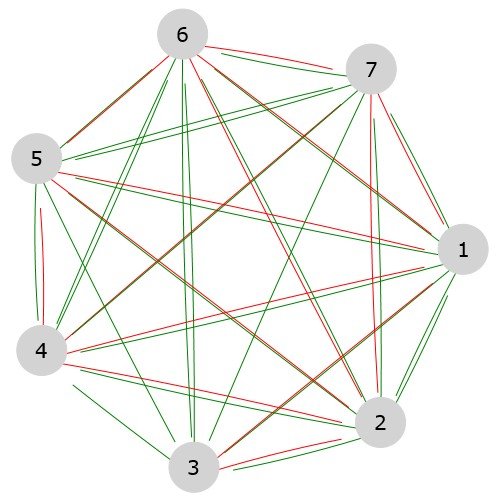
\includegraphics[width=.58\paperwidth]{raw/graph}}
	\caption{Graph visualization for Houses7}
\end{figure*}

Between each pair of vertices, up to four relations can be present:
\begin{itemize}
	\item x S y
	\item x Sc y
	\item y S x
	\item y Sc y
\end{itemize}

Relation type is marked with line color. Green is for outranking relation (S) and red for non-outranking relation (Sc). So relation x S y will be drawn as green line between this two vertices.

All arcs are directed. Direction of arc is marked with line end. Lines ends before target vertex. So x S y relation will be drawn as line from x vertex to y vertex with line ending slightly before y.

To improve arcs visibility, only up to two arcs are drawn between vertices. If verticles contain relations: x S y, x Sc y - they will be replaced with one line with gray color. Same reduction is made for y S x, y Sc x.

You can navigate on graph by using scrollbars, zoom in and zoom out by mouse wheel. You can also drag vertices to change their position. If you click on vertex, it will be selected and summary for arcs will be displayed in tab below. All arcs weights can be displayed there (if they exists) in square brackets.

\begin{figure*}[!ht] 
	\centering
	\makebox[\textwidth]{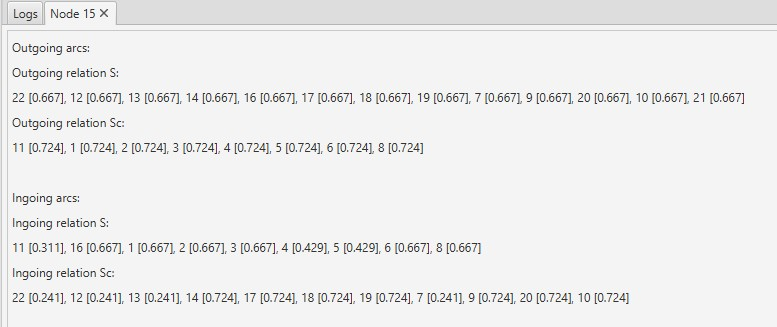
\includegraphics[width=.7\paperwidth]{raw/graph-arcs}}
	\caption{Vertex arcs for NotebooksVCcF with weights}
\end{figure*}


\vfill\newpage